\documentclass[12pt,a4paper]{article}

% ============================================
% PAQUETES
% ============================================
\usepackage[utf8]{inputenc}
\usepackage{graphicx}
\usepackage{float}
\usepackage{amsmath}
\usepackage{amssymb}
\usepackage{booktabs}
\usepackage{hyperref}
\usepackage{geometry}
\usepackage{caption}
\usepackage{subcaption}
\usepackage{listings}
\usepackage{xcolor}
\usepackage{fancyhdr}
\usepackage{titlesec}
\usepackage{enumitem}
\usepackage{longtable}
\usepackage{multirow}

% ============================================
% CONFIGURACIÓN
% ============================================
\geometry{margin=2.5cm}
\hypersetup{
    colorlinks=true,
    linkcolor=blue,
    filecolor=magenta,      
    urlcolor=cyan,
    pdftitle={Análisis de Patrones de Ventas},
}

\pagestyle{fancy}
\fancyhf{}
\rhead{Análisis de Patrones de Ventas}
\lhead{Proyecto BI}
\rfoot{Página \thepage}

\lstset{
    basicstyle=\ttfamily\small,
    breaklines=true,
    frame=single,
    backgroundcolor=\color{gray!10},
}

% ============================================
% PORTADA
% ============================================
\begin{document}

\begin{titlepage}
    \centering
    \vspace*{2cm}
    
    {\Huge\bfseries Análisis de Patrones de Ventas\\[0.5cm]}
    {\Large Reto Análisis Multivariado para Ciencia de Datos (MA2003B)\\[2cm]}
    
    \vspace{1cm}
    
    {\large\textbf{Integrantes del Equipo:}}\\[0.5cm]
    \begin{tabular}{ll}
        \textbf{Nombre:} & Marcos Saade Romano \\
        \textbf{Matrícula:} & A01784220 \\[0.3cm]
        \textbf{Nombre:} & Samuel Oropeza García \\
        \textbf{Matrícula:} & A01660110 \\[0.3cm]
        \textbf{Nombre:} & Gabriel Masri Arakindji \\
        \textbf{Matrícula:} & A01666353 \\[0.3cm]
        \textbf{Nombre:} & Aquiba Benarroch Serfaty \\
        \textbf{Matrícula:} & A01784240 \\
    \end{tabular}
    
    \vfill
    
    {\large Diciembre 2025}
    
\end{titlepage}

% ============================================
% ÍNDICE
% ============================================
\tableofcontents
\newpage

% ============================================
% 1. RESUMEN EJECUTIVO
% ============================================
\section{Resumen Ejecutivo}

Este proyecto presenta un análisis integral de los patrones de ventas de un negocio de retail, con el objetivo de identificar tendencias, estacionalidades y oportunidades de optimización. El análisis se enfoca en tres áreas principales:

\begin{enumerate}
    \item \textbf{Análisis Exploratorio de Datos (EDA):} Identificación de patrones temporales, comportamiento por categoría y región, y análisis de métodos de pago.
    \item \textbf{Segmentación mediante Clustering:} Agrupación de productos y zonas basada en patrones de demanda utilizando K-Means con selección óptima de clusters.
    \item \textbf{Modelado Predictivo:} Predicción de demanda semanal utilizando LightGBM con optimización de hiperparámetros mediante Optuna, y medias móviles para regiones con menor volumen de datos.
\end{enumerate}

Los principales hallazgos incluyen la identificación de ciclos de ventas de 2 a 8 semanas, diferencias significativas en comportamiento de compra por región (10\% de variación en gasto promedio por cliente), y la construcción de un modelo predictivo con capacidad de anticipar demanda semanal por región y categoría.

% ============================================
% 2. OBJETIVO
% ============================================
\section{Objetivo}

El objetivo principal de este proyecto es analizar los patrones y ciclicidades de ventas para:

\begin{itemize}
    \item Detectar tendencias y estacionalidad por zona, sector y categoría.
    \item Anticipar demanda a corto y mediano plazo mediante modelos predictivos.
    \item Proporcionar insights accionables para la planificación comercial.
\end{itemize}

\subsection{KPIs Analizados}
\begin{itemize}
    \item Ventas totales (monto y cantidad)
    \item Ticket promedio
    \item Participación por categoría y región
    \item Distribución por método de pago
    \item Variación mensual y semanal de ventas
\end{itemize}

% ============================================
% 3. DATOS Y ALCANCE
% ============================================
\section{Datos y Alcance}

\subsection{Fuente de Datos}
Los datos provienen de un dataset de Kaggle que contiene información de ventas de un negocio de retail en Argentina. El dataset incluye las siguientes tablas:

\begin{itemize}
    \item \texttt{ventas.csv}: Registro de transacciones individuales
    \item \texttt{productos.csv}: Catálogo de productos con precios
    \item \texttt{categorias.csv}: Clasificación de productos
    \item \texttt{clientes.csv}: Información de clientes y regiones
    \item \texttt{metodos\_pago.csv}: Métodos de pago disponibles
\end{itemize}

\subsection{Cobertura Temporal}
El dataset contiene datos de aproximadamente \textbf{11 meses} (febrero a diciembre). Es importante notar que:

\begin{itemize}
    \item Se eliminó enero del análisis debido a que los datos comenzaban el día 31, lo cual no es representativo del mes completo.
    \item Contar con datos de un solo año limita el análisis de patrones estacionales interanuales. Las tendencias mensuales observadas pueden estar influenciadas por ruido y no necesariamente representan patrones recurrentes.
\end{itemize}

\subsection{Decisión sobre Granularidad Temporal}
Dado que únicamente contamos con datos de un año, decidimos realizar el análisis de ventas a nivel \textbf{semanal} en lugar de diario. Esta decisión se basa en:

\begin{enumerate}
    \item Es impráctico optimizar inventarios y fuerza de ventas a nivel diario.
    \item La agregación semanal reduce el ruido en los datos.
    \item Dependiendo de los objetivos reales del negocio, es fácil ajustar nuestros modelos para predecir demanda cada $n$ semanas o meses (condicional en tener datos suficientes).
\end{enumerate}

\subsection{Regiones Geográficas}
El análisis cubre 6 regiones de Argentina:
\begin{itemize}
    \item Buenos Aires
    \item Centro
    \item Cuyo
    \item NEA (Noreste Argentino)
    \item NOA (Noroeste Argentino)
    \item Patagonia
\end{itemize}

\subsection{Categorías de Productos}
Las categorías analizadas incluyen:
\begin{itemize}
    \item Carnicería
    \item Frutas y Verduras
    \item Galletitas y Snacks
    \item Lácteos
    \item Panadería
\end{itemize}

% ============================================
% 4. LIMPIEZA Y FEATURE ENGINEERING
% ============================================
\section{Limpieza de Datos y Feature Engineering}

\subsection{Proceso de Limpieza}

La limpieza de datos siguió un proceso sistemático documentado en la bitácora de decisiones:

\subsubsection{Eliminación de Duplicados}
Se identificaron y eliminaron 29 registros duplicados en el campo \texttt{ID\_Venta} (de 3029 a 3000 registros únicos).

\subsubsection{Integración de Datos}
Se integraron las tablas auxiliares al dataset principal de ventas:
\begin{itemize}
    \item Categorías de productos
    \item Regiones de clientes
    \item Métodos de pago
    \item Precios unitarios
\end{itemize}

\subsubsection{Corrección de Formatos}
\begin{itemize}
    \item Conversión de precios del formato europeo (coma como separador decimal) al formato estándar.
    \item Estandarización de nombres de columnas (eliminación de acentos).
    \item Conversión de fechas al formato datetime.
\end{itemize}

\subsubsection{Tratamiento de Outliers}
Se identificaron y eliminaron outliers en el monto de venta utilizando el método IQR (Rango Intercuartílico):
\begin{equation}
    \text{Outlier si: } x < Q_1 - 1.5 \times IQR \quad \text{o} \quad x > Q_3 + 1.5 \times IQR
\end{equation}

Los outliers identificados mostraban montos idénticos y no correspondían a fechas especiales, sugiriendo posibles errores en la recolección de datos.

% GRÁFICA DE OUTLIERS
\begin{figure}[H]
    \centering
    \includegraphics[width=0.8\textwidth]{images/outliers.png}
    \caption{Identificación de outliers en monto de venta utilizando IQR}
    \label{fig:outliers}
\end{figure}

\subsection{Feature Engineering}

Se implementó una clase modular \texttt{FeatureEngineer} en Python para la creación sistemática de características:

\subsubsection{Variables Temporales}
\begin{itemize}
    \item Semana del año
    \item Mes
    \item Día de la semana
\end{itemize}

\subsubsection{Variables de Lag}
\begin{itemize}
    \item \texttt{ventas\_categoria\_lag\_1}: Ventas de la categoría en el período anterior
    \item \texttt{ventas\_region\_lag\_1}: Ventas de la región en el período anterior
    \item \texttt{cantidad\_lag\_1}: Cantidad vendida en el período anterior (por categoría y región)
\end{itemize}

\subsubsection{Medias Móviles (Rolling Features)}
Se calcularon medias y desviaciones estándar móviles para ventanas de 3, 7, 14 y 30 días, así como ventanas semanales (2-6 semanas):
\begin{itemize}
    \item \texttt{ventas\_categoria\_rolling\_mean\_\{n\}}: Media móvil de $n$ períodos por categoría
    \item \texttt{ventas\_region\_rolling\_mean\_\{n\}}: Media móvil de $n$ períodos por región
    \item \texttt{ventas\_categoria\_rolling\_std\_\{n\}}: Volatilidad móvil por categoría
    \item \texttt{ventas\_region\_rolling\_std\_\{n\}}: Volatilidad móvil por región
\end{itemize}

\subsubsection{Variables de Interacción}
\begin{itemize}
    \item Ratios cantidad/media móvil
    \item Ratios entre diferentes ventanas temporales
    \item Combinaciones de media y volatilidad
\end{itemize}

\textbf{Nota:} Los valores NaN generados por las medias móviles y lags no fueron rellenados, ya que los modelos utilizados (LightGBM) manejan nativamente valores faltantes.

% ============================================
% 5. ANÁLISIS EXPLORATORIO
% ============================================
\section{Análisis Exploratorio de Datos (EDA)}

\subsection{Distribución de Ventas por Categoría}

El análisis reveló diferencias significativas entre el monto vendido y la cantidad de unidades por categoría:

\begin{itemize}
    \item \textbf{Carnicería} lidera en monto de ventas debido a precios unitarios más altos.
    \item \textbf{Frutas y Verduras} lidera en cantidad de unidades vendidas.
\end{itemize}

Esto tiene implicaciones importantes para proyecciones financieras (donde carnicería tiene mayor peso) versus gestión de inventario físico (donde frutas y verduras demandan más espacio y rotación).

% GRÁFICA DE VENTAS POR CATEGORÍA
\begin{figure}[H]
    \centering
    \includegraphics[width=0.9\textwidth]{images/ventas_categoria.png}
    \caption{Comparación de ventas por categoría: monto vs cantidad}
    \label{fig:ventas_categoria}
\end{figure}

\subsection{Análisis de Correlaciones}

Se analizó la relación entre precio unitario, cantidad y monto de venta:

\begin{itemize}
    \item Correlación Precio-Monto: 0.71
    \item Correlación Cantidad-Monto: 0.62
    \item Correlación Precio-Cantidad: 0.01
\end{itemize}

\textbf{Hallazgo:} El precio unitario influye más en el monto de venta que la cantidad. Además, un precio mayor no reduce la cantidad comprada (correlación prácticamente nula), sugiriendo baja elasticidad precio en las categorías analizadas.

% GRÁFICA DE CORRELACIÓN
\begin{figure}[H]
    \centering
    \includegraphics[width=0.6\textwidth]{images/correlacion_heatmap.png}
    \caption{Matriz de correlación entre variables principales}
    \label{fig:correlacion}
\end{figure}

\subsection{Análisis por Región}

Buenos Aires es la región con mayores ventas tanto en monto como en cantidad, mientras que NOA presenta las menores ventas. Sin embargo, al normalizar por número de clientes:

\begin{itemize}
    \item \textbf{Cuyo:} Mayor gasto promedio por cliente (33.3)
    \item \textbf{Patagonia:} Menor gasto promedio por cliente (29.7)
    \item Diferencia de aproximadamente 10\% entre regiones extremas
\end{itemize}

% GRÁFICA DE VENTAS POR REGIÓN
\begin{figure}[H]
    \centering
    \includegraphics[width=0.9\textwidth]{images/ventas_region.png}
    \caption{Distribución de ventas por región y gasto promedio por cliente}
    \label{fig:ventas_region}
\end{figure}

\subsection{Patrones Temporales}

\subsubsection{Análisis de Ciclicidad}
Utilizando análisis de medias móviles y detección de picos (\texttt{scipy.signal.find\_peaks}):

\begin{itemize}
    \item Distancia promedio entre picos (MA7): Variable, rango de 7-60 días
    \item Distancia promedio entre picos (MA14): Mayor estabilidad, ciclos de ~30-45 días
\end{itemize}

% GRÁFICA DE MEDIAS MÓVILES
\begin{figure}[H]
    \centering
    \includegraphics[width=0.9\textwidth]{images/medias_moviles.png}
    \caption{Series temporales de ventas con medias móviles de 7, 14 y 30 días}
    \label{fig:medias_moviles}
\end{figure}

\subsubsection{Estacionalidad Mensual}
Se observó variación en las ventas por mes, aunque con la limitación de contar con datos de un solo año. Los meses con desviaciones positivas respecto al promedio sugieren oportunidades para promociones y ajuste de inventarios.

% GRÁFICA DE ESTACIONALIDAD
\begin{figure}[H]
    \centering
    \includegraphics[width=0.8\textwidth]{images/estacionalidad.png}
    \caption{Porcentaje de desviación del promedio mensual de ventas}
    \label{fig:estacionalidad}
\end{figure}

\subsection{Métodos de Pago}

\textbf{Hallazgos principales:}
\begin{itemize}
    \item \textbf{Mercado Pago} es el método de pago dominante en todas las regiones y categorías.
    \item En verano se observa un aumento en el uso de transferencias bancarias.
    \item La categoría "Galletitas y Snacks" muestra mayor diversificación en métodos de pago.
\end{itemize}

% GRÁFICA DE MÉTODOS DE PAGO
\begin{figure}[H]
    \centering
    \includegraphics[width=0.9\textwidth]{images/metodos_pago.png}
    \caption{Distribución de ventas por método de pago y evolución temporal}
    \label{fig:metodos_pago}
\end{figure}

% ============================================
% 6. CLUSTERING
% ============================================
\section{Segmentación mediante Clustering}

\subsection{Objetivo}
Identificar grupos de productos y zonas con patrones de ventas similares para optimizar la gestión del inventario y la asignación de recursos de ventas.

\subsection{Metodología}

\subsubsection{Preparación de Datos}
\begin{enumerate}
    \item Selección de variables numéricas relevantes
    \item Estandarización mediante \texttt{StandardScaler}
    \item Tratamiento de valores faltantes mediante forward/backward fill
\end{enumerate}

\subsubsection{Variables Utilizadas}
\begin{itemize}
    \item Cantidad vendida
    \item Medias móviles de 3 y 7 días (categoría)
    \item Desviaciones estándar móviles de 3 y 7 días
    \item ID de Región
    \item ID de Categoría
\end{itemize}

\subsubsection{Selección del Número de Clusters}
Se utilizaron dos métodos complementarios:

\textbf{1. Método del Codo (Elbow Method):}
Análisis de la inercia (suma de distancias al cuadrado dentro de clusters) para identificar el punto de inflexión.

\textbf{2. Silhouette Score:}
Métrica que evalúa qué tan similar es cada punto a su propio cluster comparado con otros clusters:
\begin{equation}
    s(i) = \frac{b(i) - a(i)}{\max(a(i), b(i))}
\end{equation}
donde $a(i)$ es la distancia promedio dentro del cluster y $b(i)$ es la distancia promedio al cluster más cercano.

\textbf{Resultado:} Se seleccionaron \textbf{6 clusters} basándose en un Silhouette Score óptimo y el punto de inflexión en el gráfico de codo.

% GRÁFICA DE ELBOW Y SILHOUETTE
\begin{figure}[H]
    \centering
    \includegraphics[width=0.9\textwidth]{images/elbow_silhouette.png}
    \caption{Selección del número óptimo de clusters}
    \label{fig:elbow_silhouette}
\end{figure}

\subsection{Visualización de Clusters}

\subsubsection{Reducción de Dimensionalidad}
Se aplicó PCA (Análisis de Componentes Principales) para visualizar los clusters en dimensiones reducidas:
\begin{itemize}
    \item 4 componentes principales capturan la mayor parte de la varianza explicada
    \item Visualización en 2D y 3D para interpretación
\end{itemize}

% GRÁFICA DE CLUSTERS PCA
\begin{figure}[H]
    \centering
    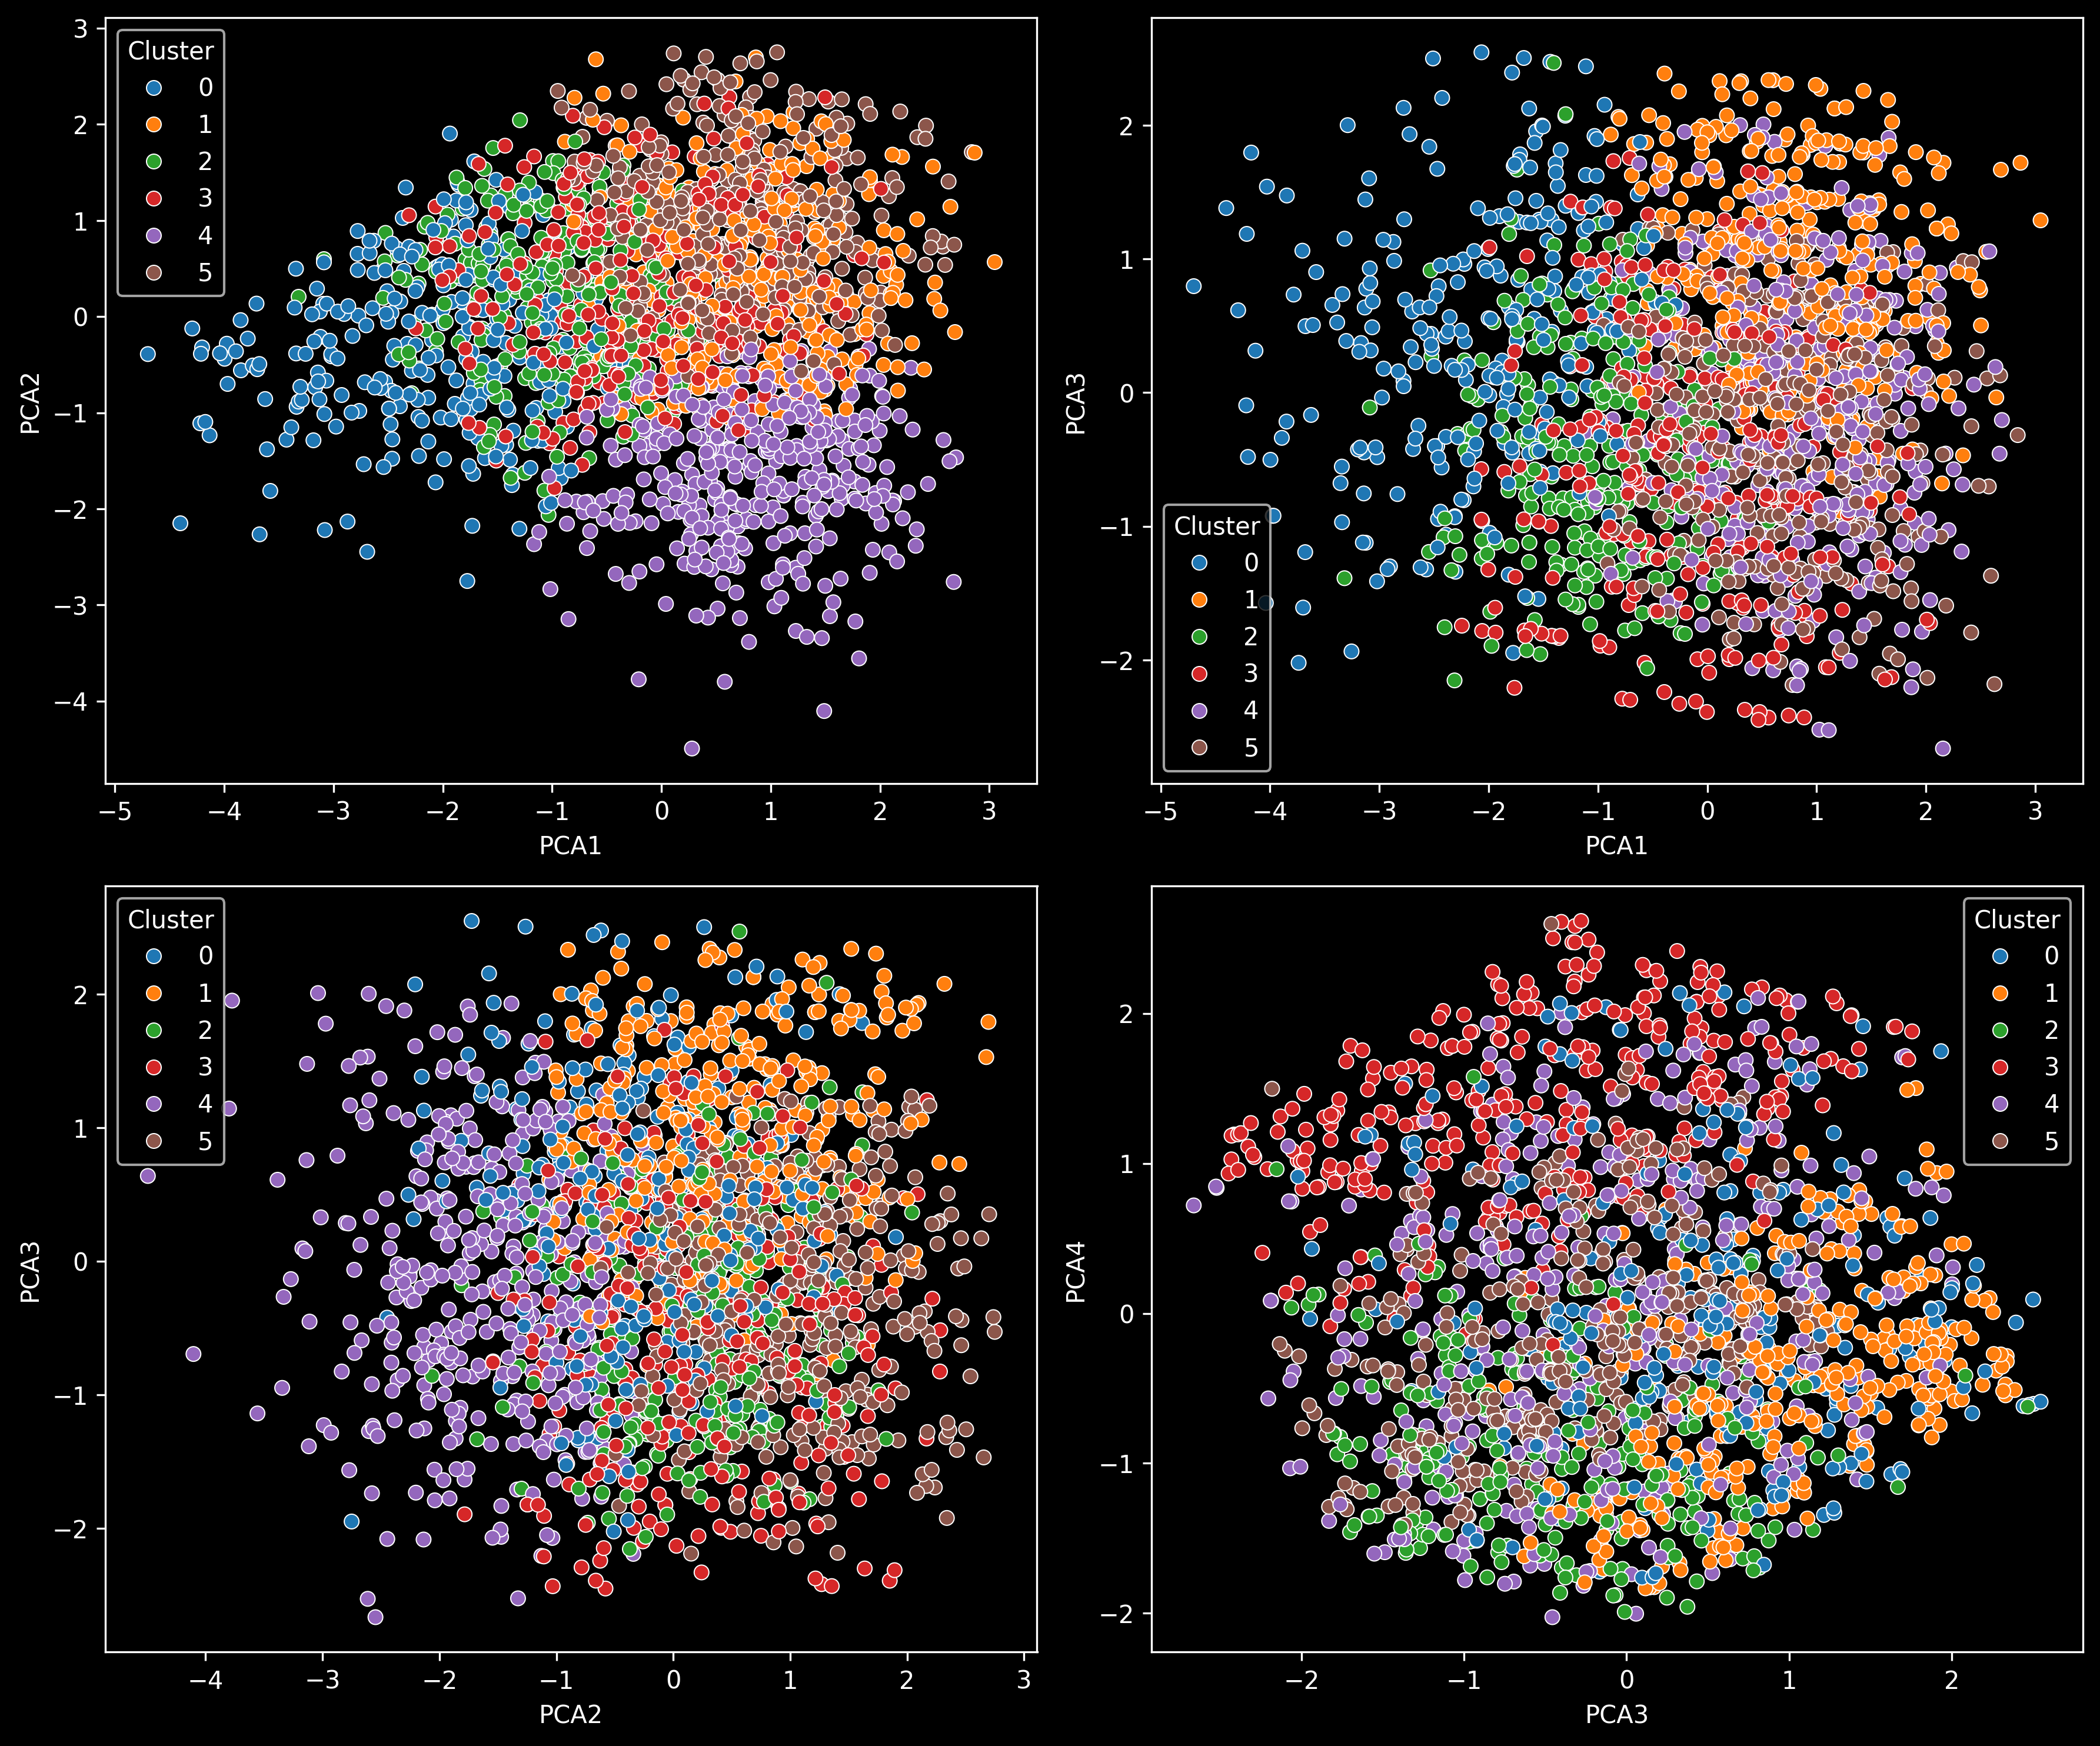
\includegraphics[width=0.9\textwidth]{images/clusters_pca.png}
    \caption{Clusters proyectados en componentes principales}
    \label{fig:clusters_pca}
\end{figure}

% GRÁFICA DE CLUSTERS 3D
\begin{figure}[H]
    \centering
    \includegraphics[width=0.7\textwidth]{images/clusters_3d.png}
    \caption{Representación tridimensional de clusters}
    \label{fig:clusters_3d}
\end{figure}

\subsection{Interpretación de Clusters}

Los 6 clusters identificados representan diferentes patrones de demanda basados en:
\begin{itemize}
    \item Nivel de cantidad vendida
    \item Volatilidad (variabilidad en ventas)
    \item Comportamiento regional
    \item Tendencias en medias móviles
\end{itemize}

Estos clusters permiten diseñar estrategias diferenciadas de inventario y promociones según el comportamiento de cada segmento.

% ============================================
% 7. MODELADO PREDICTIVO
% ============================================
\section{Modelado Predictivo}

\subsection{Objetivo}
Predecir la demanda semanal por región y categoría para apoyar la planificación de inventarios y recursos.

\subsection{Estrategia de Modelado}

Dada la heterogeneidad en los datos entre regiones, se implementó una estrategia híbrida:

\begin{enumerate}
    \item \textbf{LightGBM:} Para regiones con suficiente volumen de datos (Buenos Aires, Centro, Cuyo, Patagonia)
    \item \textbf{Media Móvil:} Para regiones con menor volumen (NEA, NOA)
\end{enumerate}

\subsection{LightGBM}

\subsubsection{Justificación}
LightGBM (Light Gradient Boosting Machine) fue seleccionado por:
\begin{itemize}
    \item Manejo nativo de valores faltantes
    \item Eficiencia computacional
    \item Capacidad de capturar no linealidades
    \item Robustez ante sobreajuste mediante regularización
\end{itemize}

\subsubsection{Optimización de Hiperparámetros}
Se utilizó \textbf{Optuna} con los siguientes componentes:

\begin{itemize}
    \item \textbf{Sampler:} TPE (Tree-structured Parzen Estimator)
    \item \textbf{Pruner:} MedianPruner para eliminar trials poco prometedores
    \item \textbf{Trials:} 50 iteraciones
\end{itemize}

\textbf{Hiperparámetros optimizados:}
\begin{itemize}
    \item Learning rate: 0.01 - 0.3 (escala logarítmica)
    \item Número de hojas: 20 - 256
    \item Profundidad máxima: 3 - 12
    \item Datos mínimos por hoja: 5 - 50
    \item Feature fraction: 0.6 - 1.0
    \item Bagging fraction: 0.6 - 1.0
    \item Regularización L1 y L2
\end{itemize}

\subsubsection{Validación Temporal}
Se implementó \textbf{TimeSeriesSplit} con 5 folds para respetar la estructura temporal de los datos y evitar fuga de información del futuro:

\begin{equation}
    \text{Fold } k: \text{Train} = [0, t_k], \quad \text{Val} = [t_k+1, t_{k+1}]
\end{equation}

\subsection{Media Móvil para NEA y NOA}

Para las regiones con menor volumen de datos, se utilizó un modelo de media móvil con optimización del parámetro $n$ (número de semanas):

\begin{equation}
    \hat{y}_t = \frac{1}{n} \sum_{i=1}^{n} y_{t-i}
\end{equation}

Se evaluaron valores de $n$ de 1 a 16, seleccionando el que minimiza el RMSE en validación temporal.

% GRÁFICA DE OPTIMIZACIÓN MA
\begin{figure}[H]
    \centering
    \includegraphics[width=0.7\textwidth]{images/ma_optimization.png}
    \caption{Selección del parámetro n óptimo para media móvil}
    \label{fig:ma_optimization}
\end{figure}

\subsection{Métricas de Evaluación}

\begin{itemize}
    \item \textbf{RMSE (Root Mean Square Error):} Métrica principal
    \begin{equation}
        RMSE = \sqrt{\frac{1}{n}\sum_{i=1}^{n}(y_i - \hat{y}_i)^2}
    \end{equation}
    \item \textbf{MAE (Mean Absolute Error):} Para interpretabilidad
    \item \textbf{Early Stopping:} 50 rounds sin mejora
\end{itemize}

\subsection{Resultados}

El modelo final genera predicciones para cada combinación de región, categoría y semana:

% GRÁFICA DE PREDICCIONES POR REGIÓN
\begin{figure}[H]
    \centering
    \includegraphics[width=0.9\textwidth]{images/predicciones_region.png}
    \caption{Comparación de predicciones LGBM/MA vs cantidad semanal real}
    \label{fig:predicciones}
\end{figure}

Los resultados muestran que el modelo captura las tendencias generales de demanda, con mejor desempeño en regiones con mayor volumen de datos.

% ============================================
% 8. LIMITACIONES Y TRABAJO FUTURO
% ============================================
\section{Limitaciones y Trabajo Futuro}

\subsection{Limitaciones del Análisis Actual}

\subsubsection{Datos Temporales Limitados}
Contar con datos de solamente un año introduce ruido significativo al análisis:
\begin{itemize}
    \item Las tendencias mensuales observadas pueden no ser representativas de patrones recurrentes.
    \item No es posible validar estacionalidad interanual.
    \item Eventos atípicos del año analizado pueden sesgar las conclusiones.
\end{itemize}

\subsubsection{Datos Faltantes para Optimización Avanzada}
\textbf{No es posible realizar optimización de fuerza de ventas o inventarios} sin datos adicionales como:
\begin{itemize}
    \item Volumen físico de cada producto
    \item Costos de almacenamiento
    \item Costos de transporte
    \item Capacidad de almacenamiento por ubicación
    \item Tiempos de reposición (lead times)
    \item Márgenes de ganancia por producto
\end{itemize}

\subsubsection{Granularidad del Análisis}
El análisis actual no permite:
\begin{itemize}
    \item Análisis a nivel de SKU individual
    \item Elasticidad de precios (precios fijos en el dataset)
    \item Correlación con eventos externos (promociones, competencia, clima)
\end{itemize}

\subsection{Trabajo Futuro}

\subsubsection{Iteración 1: Datos Adicionales}
En una iteración futura, sería valioso incorporar:
\begin{itemize}
    \item Datos históricos de múltiples años
    \item Información de costos operativos
    \item Datos de inventario físico
    \item Información de capacidad logística
\end{itemize}

\subsubsection{Iteración 2: Optimización Avanzada}
Con los datos adicionales, se podrían implementar:
\begin{itemize}
    \item Modelos de optimización de inventario (EOQ, políticas s-S)
    \item Asignación óptima de fuerza de ventas por región
    \item Simulación de escenarios de demanda
    \item Optimización de rutas de distribución
\end{itemize}

\subsubsection{Flexibilidad del Modelo}
El framework desarrollado permite fácilmente:
\begin{itemize}
    \item Ajustar la granularidad temporal (predicciones cada $n$ semanas o meses)
    \item Incorporar nuevas variables predictoras
    \item Reentrenar con datos actualizados
\end{itemize}

% ============================================
% 9. CONCLUSIONES Y RECOMENDACIONES
% ============================================
\section{Conclusiones y Recomendaciones}

\subsection{Principales Hallazgos}

\begin{enumerate}
    \item \textbf{Patrones de Demanda:} Se identificaron ciclos de ventas de 2-8 semanas con variabilidad significativa.
    
    \item \textbf{Diferencias Regionales:} Cuyo presenta el mayor gasto promedio por cliente, mientras que Patagonia el menor (diferencia del 10\%).
    
    \item \textbf{Métodos de Pago:} Mercado Pago domina el mercado con incremento de transferencias en verano.
    
    \item \textbf{Categorías:} Carnicería genera mayor monto pero Frutas y Verduras mayor volumen.
    
    \item \textbf{Modelo Predictivo:} LightGBM optimizado con Optuna proporciona predicciones semanales robustas.
\end{enumerate}

\subsection{Recomendaciones de Negocio}

\subsubsection{Corto Plazo}
\begin{itemize}
    \item Utilizar las predicciones semanales para ajustar pedidos de reposición.
    \item Planificar promociones en períodos de menor demanda identificados.
    \item Reforzar opciones de Mercado Pago y transferencias según temporada.
\end{itemize}

\subsubsection{Mediano Plazo}
\begin{itemize}
    \item Recolectar datos de costos para habilitar optimización de inventarios.
    \item Expandir el horizonte temporal de datos para validar patrones estacionales.
    \item Implementar monitoreo continuo de predicciones vs. realidad.
\end{itemize}

\subsubsection{Largo Plazo}
\begin{itemize}
    \item Desarrollar sistema automatizado de reposición basado en predicciones.
    \item Integrar datos externos (clima, eventos, competencia) al modelo.
    \item Implementar segmentación de clientes para marketing personalizado.
\end{itemize}

% ============================================
% 10. ESTRUCTURA DEL REPOSITORIO
% ============================================
\section{Estructura del Repositorio}

El código del proyecto está organizado siguiendo mejores prácticas:

\begin{lstlisting}
AnalisisVentas/
|-- data_raw/           # Datos originales
|   |-- categorias.csv
|   |-- clientes.csv
|   |-- metodos_pago.csv
|   |-- productos.csv
|   |-- ventas.csv
|
|-- data_clean/         # Datos procesados
|   |-- ventas_clean.csv
|   |-- data_fe.csv
|   |-- data_fe_clusters.csv
|   |-- data_modelado.csv
|   |-- data_con_predicciones.csv
|
|-- notebooks/          # Analisis exploratorio y modelado
|   |-- EDA.ipynb
|   |-- clustering.ipynb
|   |-- modelado-predictivo.ipynb
|   |-- best_lgbm_params.json
|
|-- src/                # Codigo fuente modular
|   |-- feature_engineering.py
|
|-- reports/            # Reportes y documentacion
|   |-- bitacora_desiciones.md
|   |-- reporte.tex
|
|-- README.md           # Instrucciones de ejecucion
\end{lstlisting}

\subsection{Reproducibilidad}
\begin{itemize}
    \item Semillas aleatorias fijadas (seed=42) para reproducibilidad
    \item Hiperparámetros óptimos guardados en JSON
    \item Pipeline de feature engineering modular y reutilizable
\end{itemize}

% ============================================
% APÉNDICE
% ============================================
\appendix
\section{Bitácora de Decisiones}

\subsection{Limpieza de Datos}

\subsubsection{Eliminación de Duplicados}
\begin{itemize}
    \item Identificamos 29 registros duplicados en \texttt{ID\_Venta} (de 3029 a 3000 registros únicos)
    \item \textbf{Decisión:} Eliminamos duplicados usando \texttt{drop\_duplicates(subset='ID\_Venta')}
    \item \textbf{Justificación:} Los duplicados representan errores de registro, no transacciones válidas
\end{itemize}

\subsubsection{Integración de Tablas}
\begin{itemize}
    \item Agregamos al dataset ventas las regiones de acuerdo al ID de cliente
    \item Agregamos las categorías de acuerdo al ID de producto
    \item Agregamos precio unitario desde la tabla de productos
    \item Agregamos método de pago desde la tabla de métodos de pago
    \item \textbf{Justificación:} Consolidar toda la información relevante en un solo DataFrame
\end{itemize}

\subsubsection{Estandarización de Formatos}
\begin{itemize}
    \item Renombramos columnas para eliminar acentos (\texttt{Categoría} $\rightarrow$ \texttt{Categoria})
    \item Convertimos \texttt{Precio\_Unitario} de formato europeo (coma) a estándar (punto)
    \item Convertimos columna \texttt{Fecha} a formato datetime con \texttt{dayfirst=True}
    \item \textbf{Justificación:} Evitar problemas de encoding y facilitar manipulación programática
\end{itemize}

\subsubsection{Tratamiento de Período Temporal}
\begin{itemize}
    \item Eliminamos enero por empezar en el día 31 (no representativo del mes)
    \item \textbf{Decisión:} \texttt{df = df[df['Fecha'].dt.month != 1]}
    \item \textbf{Justificación:} Un solo día de enero sesgaría cualquier análisis mensual
\end{itemize}

\subsubsection{Tratamiento de Outliers}
\begin{itemize}
    \item Identificamos outliers en \texttt{Monto\_Venta} usando el método IQR
    \item Los outliers detectados tenían montos idénticos y no correspondían a fechas especiales
    \item \textbf{Decisión:} Eliminamos los outliers por categoría
    \item \textbf{Justificación:} En retail es importante predecir outliers, pero un análisis reveló que parecen ser aleatorios (sin periodicidad clara ni correspondencia con fechas importantes)
\end{itemize}

\subsubsection{Creación de Tickets}
\begin{itemize}
    \item Creamos \texttt{ID\_Ticket} agrupando por \texttt{ID\_Cliente} y \texttt{Fecha}
    \item Identificamos solo 44 de 3000 tickets con múltiples productos
    \item \textbf{Nota:} Esta baja proporción debe validarse con el equipo de datos
\end{itemize}

\subsection{Feature Engineering}

\subsubsection{Variables Creadas}
\begin{itemize}
    \item \textbf{Monto de Venta:} \texttt{Cantidad * Precio\_Unitario}
    \item \textbf{Variables Temporales:} semana, mes, día de la semana
    \item \textbf{Variables de Lag:} ventas\_categoria\_lag\_1, ventas\_region\_lag\_1, cantidad\_lag\_1
    \item \textbf{Medias Móviles:} Ventanas de 3, 7, 14, 30 días y 2-6 semanas (media y desviación estándar)
    \item \textbf{Variables de Interacción:} Ratios cantidad/media móvil, ratios entre ventanas
    \item \textbf{Codificación:} ID\_Region como variable numérica
\end{itemize}

\subsubsection{Decisiones Clave}
\begin{itemize}
    \item Usamos \texttt{shift(1)} antes del rolling para evitar data leakage
    \item No rellenamos NaNs generados por medias móviles (LightGBM los maneja nativamente)
\end{itemize}

\subsection{Clustering}
\begin{itemize}
    \item \textbf{Preparación:} Estandarización con StandardScaler, forward/backward fill para NaNs
    \item \textbf{Variables:} Cantidad, medias móviles (3 y 7 días), volatilidad, ID\_Region, ID\_Categoria
    \item \textbf{Selección de k:} 6 clusters basado en método del codo y Silhouette Score
    \item \textbf{Visualización:} PCA con 4 componentes para reducción de dimensionalidad
\end{itemize}

\subsection{Modelado Predictivo}
\begin{itemize}
    \item \textbf{Estrategia Híbrida:} LightGBM para regiones con volumen suficiente, Media Móvil para NEA y NOA
    \item \textbf{Variable Objetivo:} Cantidad\_Semanal (agregada por semana, región y categoría)
    \item \textbf{Validación:} TimeSeriesSplit con 5 folds (respeta orden temporal)
    \item \textbf{Optimización LGBM:} Optuna con 50 trials, TPE sampler, MedianPruner
    \item \textbf{Optimización MA:} Evaluación de ventanas 1-16 semanas, selección por RMSE mínimo
    \item \textbf{Reproducibilidad:} seed=42 en todos los componentes
\end{itemize}

\subsection{Decisiones de Alcance}
\begin{itemize}
    \item \textbf{No realizamos:} Optimización de fuerza de ventas ni inventarios (faltan datos de costos)
    \item \textbf{Análisis no realizados:} Elasticidad de precios (precios fijos), estacionalidad interanual (solo un año)
    \item \textbf{Trabajo futuro:} Datos de costos, múltiples años, datos externos (clima, eventos)
\end{itemize}

% ============================================
% ANÁLISIS DE FEATURE IMPORTANCE
% ============================================
\section{Análisis de Importancia de Variables}

El modelo LightGBM proporciona métricas de importancia de variables que permiten entender qué características tienen mayor poder predictivo para la demanda semanal.

\subsection{Métricas de Importancia}

Se analizaron dos métricas complementarias:

\begin{itemize}
    \item \textbf{Importance by Gain:} Suma de la ganancia (reducción de pérdida) aportada por cada variable en todos los splits donde fue utilizada. Variables con mayor gain contribuyen más a la precisión del modelo.
    \item \textbf{Importance by Split:} Número de veces que cada variable fue utilizada para hacer splits en los árboles. Variables con mayor split frequency son consideradas más frecuentemente por el modelo.
\end{itemize}

\subsection{Resultados}

% GRÁFICA DE FEATURE IMPORTANCE
\begin{figure}[H]
    \centering
    \includegraphics[width=0.85\textwidth]{images/feature_importance.png}
    \caption{Top 20 variables más importantes del modelo LightGBM (por ganancia)}
    \label{fig:feature_importance}
\end{figure}

\subsection{Interpretación de Resultados}

Las variables más importantes para predecir la demanda semanal incluyen:

\begin{enumerate}
    \item \textbf{Variables de tendencia reciente:} Las medias móviles de corto plazo (3-7 días) aparecen consistentemente entre las más importantes, indicando que el comportamiento reciente es un fuerte predictor de la demanda futura.
    
    \item \textbf{Variables de volatilidad:} Las desviaciones estándar móviles capturan la variabilidad en la demanda, lo cual es crucial para anticipar picos y valles.
    
    \item \textbf{Variables de lag:} Los valores rezagados confirman la autocorrelación temporal en las ventas.
    
    \item \textbf{Identificadores de región y categoría:} Su presencia indica que existen patrones diferenciados por segmento geográfico y tipo de producto.
    
    \item \textbf{Ratios de tendencia:} Las variables que comparan diferentes ventanas temporales (ej: MA7/MA14) ayudan a detectar cambios en la tendencia.
\end{enumerate}

\subsection{Implicaciones para el Negocio}

\begin{itemize}
    \item \textbf{Monitoreo de tendencias:} Es crucial dar seguimiento a las medias móviles de 3-7 días para anticipar cambios en demanda.
    \item \textbf{Segmentación:} Los patrones varían significativamente por región y categoría, justificando estrategias diferenciadas.
    \item \textbf{Gestión de volatilidad:} Las regiones/categorías con alta volatilidad requieren mayor stock de seguridad.
    \item \textbf{Actualización del modelo:} Dado el peso de variables de corto plazo, el modelo debe actualizarse frecuentemente con datos recientes.
\end{itemize}

\end{document}
